\documentclass[12pt,utf8,notheorems,compress,t]{beamer}
\usepackage{etex}

\usepackage{pgfpages}
\usepackage[export]{adjustbox}
%\setbeameroption{show notes on second screen}
%\setbeamertemplate{note page}[plain]
%\newcommand{\jnote}[2]{\only<#1>{\note{\setlength\parskip{\medskipamount}\justifying\footnotesize#2\par}}}
\newcommand{\jnote}[2]{}

% Workaround for the issue described at
% https://tex.stackexchange.com/questions/164406/beamer-using-href-in-notes.
\newcommand{\fixedhref}[2]{\makebox[0pt][l]{\hspace*{\paperwidth}\href{#1}{#2}}\href{#1}{#2}}

\usepackage[english]{babel}

\usepackage{graphbox}
\usepackage{mathtools}
\usepackage{booktabs}
\usepackage{stmaryrd}
\usepackage{amssymb}
\usepackage{array}
\usepackage{ragged2e}
\usepackage{multicol}
\usepackage{tabto}
\usepackage{xstring}
\usepackage{ifthen}
\usepackage[normalem]{ulem}
\usepackage[all]{xy}
\xyoption{rotate}
\usepackage{tikz}
\usetikzlibrary{calc,shapes,shapes.callouts,shapes.arrows,patterns,fit,backgrounds,decorations.pathmorphing,positioning}
\hypersetup{colorlinks=true}

\newcommand*\circled[1]{\tikz[baseline=(char.base)]{%
  \node[shape=circle,draw,inner sep=1pt] (char) {#1};}}

\DeclareFontFamily{U}{bbm}{}
\DeclareFontShape{U}{bbm}{m}{n}
   {  <5> <6> <7> <8> <9> <10> <12> gen * bbm
      <10.95> bbm10%
      <14.4>  bbm12%
      <17.28><20.74><24.88> bbm17}{}
\DeclareFontShape{U}{bbm}{m}{sl}
   {  <5> <6> <7> bbmsl8%
      <8> <9> <10> <12> gen * bbmsl
      <10.95> bbmsl10%
      <14.4> <17.28> <20.74> <24.88> bbmsl12}{}
\DeclareFontShape{U}{bbm}{bx}{n}
   {  <5> <6> <7> <8> <9> <10> <12> gen * bbmbx
      <10.95> bbmbx10%
      <14.4> <17.28> <20.74> <24.88> bbmbx12}{}
\DeclareFontShape{U}{bbm}{bx}{sl}
   {  <5> <6> <7> <8> <9> <10> <10.95> <12> <14.4> <17.28>%
      <20.74> <24.88> bbmbxsl10}{}
\DeclareFontShape{U}{bbm}{b}{n}
   {  <5> <6> <7> <8> <9> <10> <10.95> <12> <14.4> <17.28>%
      <20.74> <24.88> bbmb10}{}
\DeclareMathAlphabet{\mathbbm}{U}{bbm}{m}{n}
\SetMathAlphabet\mathbbm{bold}{U}{bbm}{bx}{n}


\usepackage{pifont}
\newcommand{\cmark}{\ding{51}}
\newcommand{\xmark}{\ding{55}}
\DeclareSymbolFont{extraup}{U}{zavm}{m}{n}
\DeclareMathSymbol{\varheart}{\mathalpha}{extraup}{86}

\graphicspath{{images/}}

\usepackage[protrusion=true,expansion=true]{microtype}

\setlength\parskip{\medskipamount}
\setlength\parindent{0pt}

\title{Bridging the foundational gap: updating algebraic geometry in
face of current challenges regarding formalizability, constructivity and
predicativity}
\author{Ingo Blechschmidt}
\date{November 23th, 2021}

\useinnertheme[shadow=true]{rounded}
\setbeamerfont{block title}{size={}}

\useinnertheme{rectangles}

\usecolortheme{orchid}
\usecolortheme{seahorse}
\definecolor{mypurple}{RGB}{150,0,255}
\setbeamercolor{structure}{fg=mypurple}
\definecolor{myred}{RGB}{150,0,0}
\setbeamercolor*{title}{bg=myred,fg=white}
\setbeamercolor*{titlelike}{bg=myred,fg=white}
\setbeamercolor{frame}{bg=black}

\usefonttheme{serif}
\usepackage[T1]{fontenc}
\usepackage{libertine}

% lifted from https://arxiv.org/abs/1506.08870
\DeclareFontFamily{U}{min}{}
\DeclareFontShape{U}{min}{m}{n}{<-> udmj30}{}
\newcommand\yon{\!\text{\usefont{U}{min}{m}{n}\symbol{'210}}\!}

\newcommand{\A}{\mathcal{A}}
\newcommand{\B}{\mathcal{B}}
\newcommand{\C}{\mathcal{C}}
\newcommand{\M}{\mathcal{M}}
\renewcommand{\AA}{\mathbb{A}}
\newcommand{\BB}{\mathbb{B}}
\newcommand{\pp}{\mathbbm{p}}
\newcommand{\MM}{\mathbb{M}}
\newcommand{\E}{\mathcal{E}}
\newcommand{\F}{\mathcal{F}}
\newcommand{\FF}{\mathbb{F}}
\newcommand{\G}{\mathcal{G}}
\newcommand{\J}{\mathcal{J}}
\newcommand{\GG}{\mathbb{G}}
\renewcommand{\O}{\mathcal{O}}
\newcommand{\K}{\mathcal{K}}
\newcommand{\NN}{\mathbb{N}}
\newcommand{\QQ}{\mathbb{Q}}
\newcommand{\RR}{\mathbb{R}}
\newcommand{\TT}{\mathbb{T}}
\newcommand{\PP}{\mathbb{P}}
\newcommand{\ZZ}{\mathbb{Z}}
\newcommand{\CC}{\mathbb{C}}
\renewcommand{\P}{\mathcal{P}}
\newcommand{\aaa}{\mathfrak{a}}
\newcommand{\ppp}{\mathfrak{p}}
\newcommand{\fff}{\mathfrak{f}}
\newcommand{\defeq}{\vcentcolon=}
\newcommand{\defeqv}{\vcentcolon\equiv}
\newcommand{\Sh}{\mathrm{Sh}}
\newcommand{\GL}{\mathrm{GL}}
\newcommand{\Zar}{\mathrm{Zar}}
\newcommand{\op}{\mathrm{op}}
\newcommand{\Set}{\mathrm{Set}}
\newcommand{\Eff}{\mathrm{Ef{}f}}
\newcommand{\Sch}{\mathrm{Sch}}
\newcommand{\Aff}{\mathrm{Aff}}
\newcommand{\Ring}{\mathrm{Ring}}
\newcommand{\LocRing}{\mathrm{LocRing}}
\newcommand{\LRS}{\mathrm{LRS}}
\newcommand{\Hom}{\mathrm{Hom}}
\newcommand{\Spec}{\mathrm{Spec}}
\newcommand{\lra}{\longrightarrow}
\newcommand{\RelSpec}{\operatorname{Spec}}
\renewcommand{\_}{\mathpunct{.}}
\newcommand{\?}{\,{:}\,}
\newcommand{\speak}[1]{\ulcorner\text{\textnormal{#1}}\urcorner}
\newcommand{\ul}[1]{\underline{#1}}
\newcommand{\affl}{\ensuremath{{\ul{\ensuremath{\AA}}^1}}}
\newcommand{\Ll}{\text{iff}}
\newcommand{\inv}{inv.\@}
\newcommand{\seq}[1]{\mathrel{\vdash\!\!\!_{#1}}}
\newcommand{\hg}{\mathbin{:}}  % homogeneous coordinates

\setbeamertemplate{blocks}[rounded][shadow=false]

\newenvironment{indentblock}{%
  \list{}{\leftmargin\leftmargin}%
  \item\relax
}{%
  \endlist
}

% Adapted from https://latex.org/forum/viewtopic.php?t=2251 (Stefan Kottwitz)
\newenvironment<>{hilblock}{
  \begin{center}
    \begin{minipage}{9.05cm}
      \setlength{\textwidth}{9.05cm}
      \begin{actionenv}#1
        \def\insertblocktitle{}
        \par
        \usebeamertemplate{block begin}}{
        \par
        \usebeamertemplate{block end}
      \end{actionenv}
    \end{minipage}
  \end{center}}

\newenvironment{changemargin}[2]{%
  \begin{list}{}{%
    \setlength{\topsep}{0pt}%
    \setlength{\leftmargin}{#1}%
    \setlength{\rightmargin}{#2}%
    \setlength{\listparindent}{\parindent}%
    \setlength{\itemindent}{\parindent}%
    \setlength{\parsep}{\parskip}%
  }%
  \item[]}{\end{list}}

\tikzset{
  invisible/.style={opacity=0,text opacity=0},
  visible on/.style={alt={#1{}{invisible}}},
  alt/.code args={<#1>#2#3}{%
    \alt<#1>{\pgfkeysalso{#2}}{\pgfkeysalso{#3}}}
}

\newcommand{\pointthis}[3]{%
  \tikz[remember picture,baseline]{
    \node[anchor=base,inner sep=0,outer sep=0] (#2) {#2};
    \node[visible on=#1,overlay,rectangle callout,rounded corners,callout relative pointer={(0.3cm,0.5cm)},fill=blue!20] at ($(#2.north)+(-0.1cm,-1.1cm)$) {#3};
  }%
}

\tikzset{
  invisible/.style={opacity=0,text opacity=0},
  visible on/.style={alt={#1{}{invisible}}},
  alt/.code args={<#1>#2#3}{%
    \alt<#1>{\pgfkeysalso{#2}}{\pgfkeysalso{#3}}}
}

\newcommand{\hcancel}[5]{%
  \tikz[baseline=(tocancel.base)]{
    \node[inner sep=0pt,outer sep=0pt] (tocancel) {#1};
    \draw[red!80, line width=0.4mm] ($(tocancel.south west)+(#2,#3)$) -- ($(tocancel.north east)+(#4,#5)$);
  }%
}

\newcommand{\explain}[7]{%
  \tikz[remember picture,baseline]{
    \node[anchor=base,inner sep=2pt,outer sep=0,fill=#3,rounded corners] (label) {#1};
    \node[anchor=north,visible on=<#2>,overlay,rectangle callout,rounded corners,callout
    relative pointer={(0.0cm,0.5cm)+(0.0cm,#6)},fill=#3] at ($(label.south)+(0,-0.3cm)+(#4,#5)$) {#7};
  }%
}

\newcommand{\explainstub}[2]{%
  \tikz[remember picture,baseline]{
    \node[anchor=base,inner sep=2pt,outer sep=0,fill=#2,rounded corners] (label) {#1};
  }%
}

\newcommand{\squiggly}[1]{%
  \tikz[remember picture,baseline]{
    \node[anchor=base,inner sep=0,outer sep=0] (label) {#1};
    \draw[thick,color=red!80,decoration={snake,amplitude=0.5pt,segment
    length=3pt},decorate] ($(label.south west) + (0,-2pt)$) -- ($(label.south east) + (0,-2pt)$);
  }%
}

% Adapted from https://latex.org/forum/viewtopic.php?t=2251 (Stefan Kottwitz)
\newenvironment<>{varblock}[2]{\begin{varblockextra}{#1}{#2}{}}{\end{varblockextra}}
\newenvironment<>{varblockextra}[3]{
  \begin{center}
    \begin{minipage}{#1}
      \begin{actionenv}#4
        {\centering \hil{#2}\par}
	\def\insertblocktitle{}%\centering #2}
        \def\varblockextraend{#3}
	\usebeamertemplate{block begin}}{
        \par
        \usebeamertemplate{block end}
        \varblockextraend
      \end{actionenv}
    \end{minipage}
  \end{center}}

\setbeamertemplate{headline}{}

\setbeamertemplate{frametitle}{%
  \vskip0.5em%
  \leavevmode%
  \begin{beamercolorbox}[dp=1ex,center]{}%
    \usebeamercolor[fg]{item}{\textbf{{\Large\insertframetitle}}}
  \end{beamercolorbox}%
  \vskip-0.2em%
}

\setbeamertemplate{navigation symbols}{}

\newcounter{framenumberpreappendix}
\newcommand{\backupstart}{
  \setcounter{framenumberpreappendix}{\value{framenumber}}
}
\newcommand{\backupend}{
  \addtocounter{framenumberpreappendix}{-\value{framenumber}}
  \addtocounter{framenumber}{\value{framenumberpreappendix}}
}

\newcommand{\insertframeextra}{}
\setbeamertemplate{footline}{%
  \begin{beamercolorbox}[wd=\paperwidth,ht=2.25ex,dp=1ex,right,rightskip=1mm,leftskip=1mm]{}%
    % \inserttitle
    \hfill
    \insertframenumber\insertframeextra\,/\,\inserttotalframenumber
  \end{beamercolorbox}%
  \vskip0pt%
}


\newcommand{\hil}[1]{{\usebeamercolor[fg]{item}{\textbf{#1}}}}
\newcommand{\bad}[1]{\textcolor{red!90}{\textnormal{#1}}}

\newcommand{\bignumber}[1]{%
  \renewcommand{\insertenumlabel}{#1}\scalebox{1.2}{\!\usebeamertemplate{enumerate item}\!}
}
\newcommand{\bigheart}{
\includegraphics{heart}}

\newcommand{\subhead}[1]{{\centering\textcolor{gray}{\hrulefill}\quad\textnormal{#1}\quad\textcolor{gray}{\hrulefill}\par}}

\begin{document}

\addtocounter{framenumber}{-1}

%\setbeamertemplate{headline}{\mynav{gray}{gray}{gray}}

{\usebackgroundtemplate{\begin{minipage}{\paperwidth}\vspace*{4.95cm}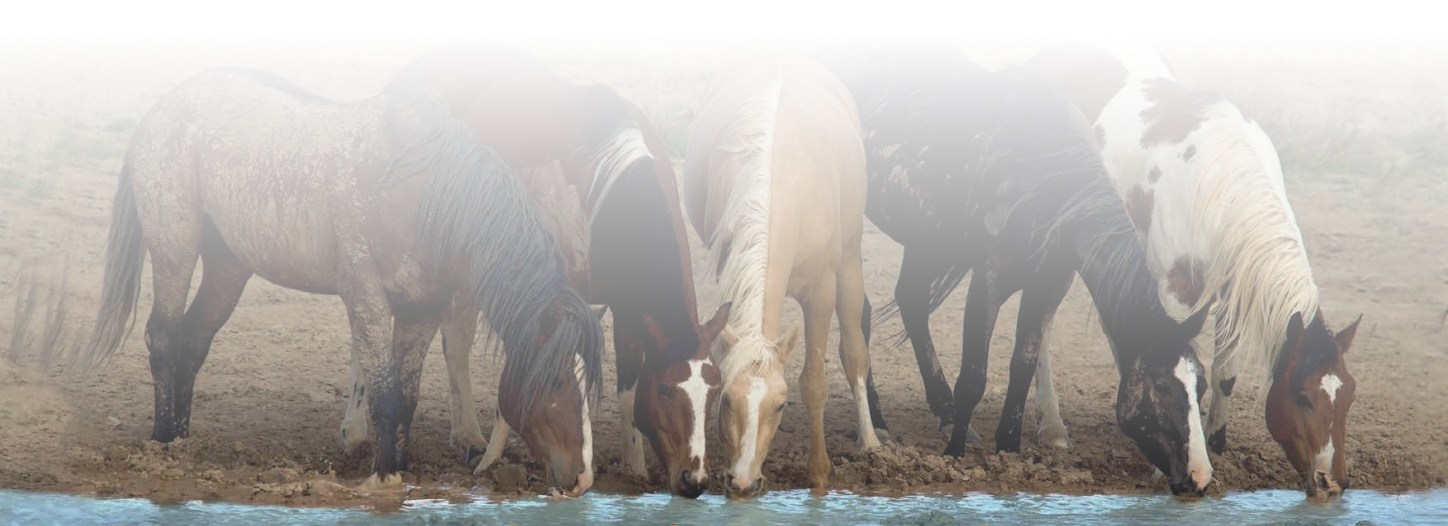
\includegraphics[width=\paperwidth]{topos-horses}\end{minipage}}
\begin{frame}[c]
  \centering

  \bigskip
  %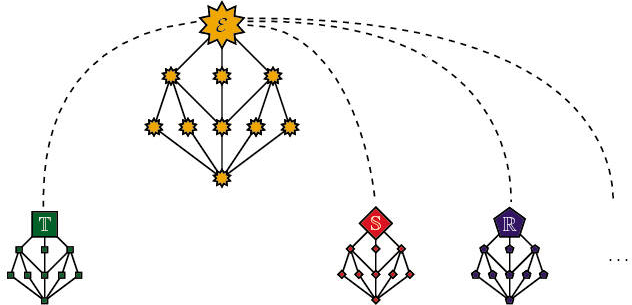
\includegraphics[height=0.32\textwidth]{olivia-lattices}
  \bigskip
  \bigskip
  \bigskip
  \bigskip

  \begin{tikzpicture}
    \def\R{8pt}
    \node (pretitle) {Bridging the foundational gap:};
    \node (title) [below of=pretitle] {\vbox{\vspace*{-0.5em}updating \hil{algebraic
    geometry} in face of \hil{current challenges} regarding
    \hil{formalizability}, \hil{constructivity} and \hil{predicativity}}};
    \begin{pgfonlayer}{background}
      \draw[decorate, very thick, draw=mypurple]
        ($(title.south west) + (\R, 0)$) arc(270:180:\R) --
        ($(title.north west) + (0, -\R)$) arc(180:90:\R) --
        ($(title.north east) + (-\R, 0)$) arc(90:0:\R) --
        ($(title.south east) + (0, \R)$) arc(0:-90:\R) --
        cycle;
    \end{pgfonlayer}
  \end{tikzpicture}

  \scriptsize
  \textit{-- an invitation --}
  \bigskip
  \bigskip
  \bigskip

  Dagstuhl Seminar 20202: \\
  Geometric Logic, Constructivisation, and Automated Theorem Proving \\
  \ \\
  November 23th, 2021
  \bigskip

  Ingo Blechschmidt \\
  University of Augsburg
  \par
\end{frame}}

{\usebackgroundtemplate{\begin{minipage}{\paperwidth}\vspace*{5.95cm}
\includegraphics[width=\paperwidth]{fr1}\end{minipage}}
\begin{frame}{Algebraic geometry in a nutshell}
  Turn \hil{commutative rings} into \hil{spaces}, and \hil{glue} those
  spaces.
  \bigskip

  \subhead{Examples}
  \begin{enumerate}
    \item $\Spec(k[X_1,\ldots,X_n]) = \AA^n$.
    \item $\Spec(k[X,Y]/(Y-X^2)) = \text{standard parabola}$.
    \item Gluing
    \begin{tikzpicture}[scale=0.2,baseline={([yshift=-.6ex]current bounding box.center)}]
      \draw (0,0) circle (1);
      \draw [fill=white] (90:1) circle (0.2);
    \end{tikzpicture}
    with
    \begin{tikzpicture}[scale=0.2,baseline={([yshift=-.6ex]current bounding box.center)}]
      \draw (0,0) circle (1);
      \draw [fill=white] (270:1) circle (0.2);
    \end{tikzpicture}
    along
    \begin{tikzpicture}[scale=0.2,baseline={([yshift=-.6ex]current bounding box.center)}]
      \draw (0,0) circle (1);
      \draw [fill=white] (90:1) circle (0.2);
      \draw [fill=white] (270:1) circle (0.2);
    \end{tikzpicture}
    yields
    $\PP^1$.
  \end{enumerate}
  \bigskip

  \subhead{Concrete results}
  Fermat's Last Theorem: For~$n \geq 3$, no positive integers satisfy
  \[ a^n + b^n = c^n. \]
\end{frame}}

{\usebackgroundtemplate{\begin{minipage}{\paperwidth}\vspace*{3.95cm}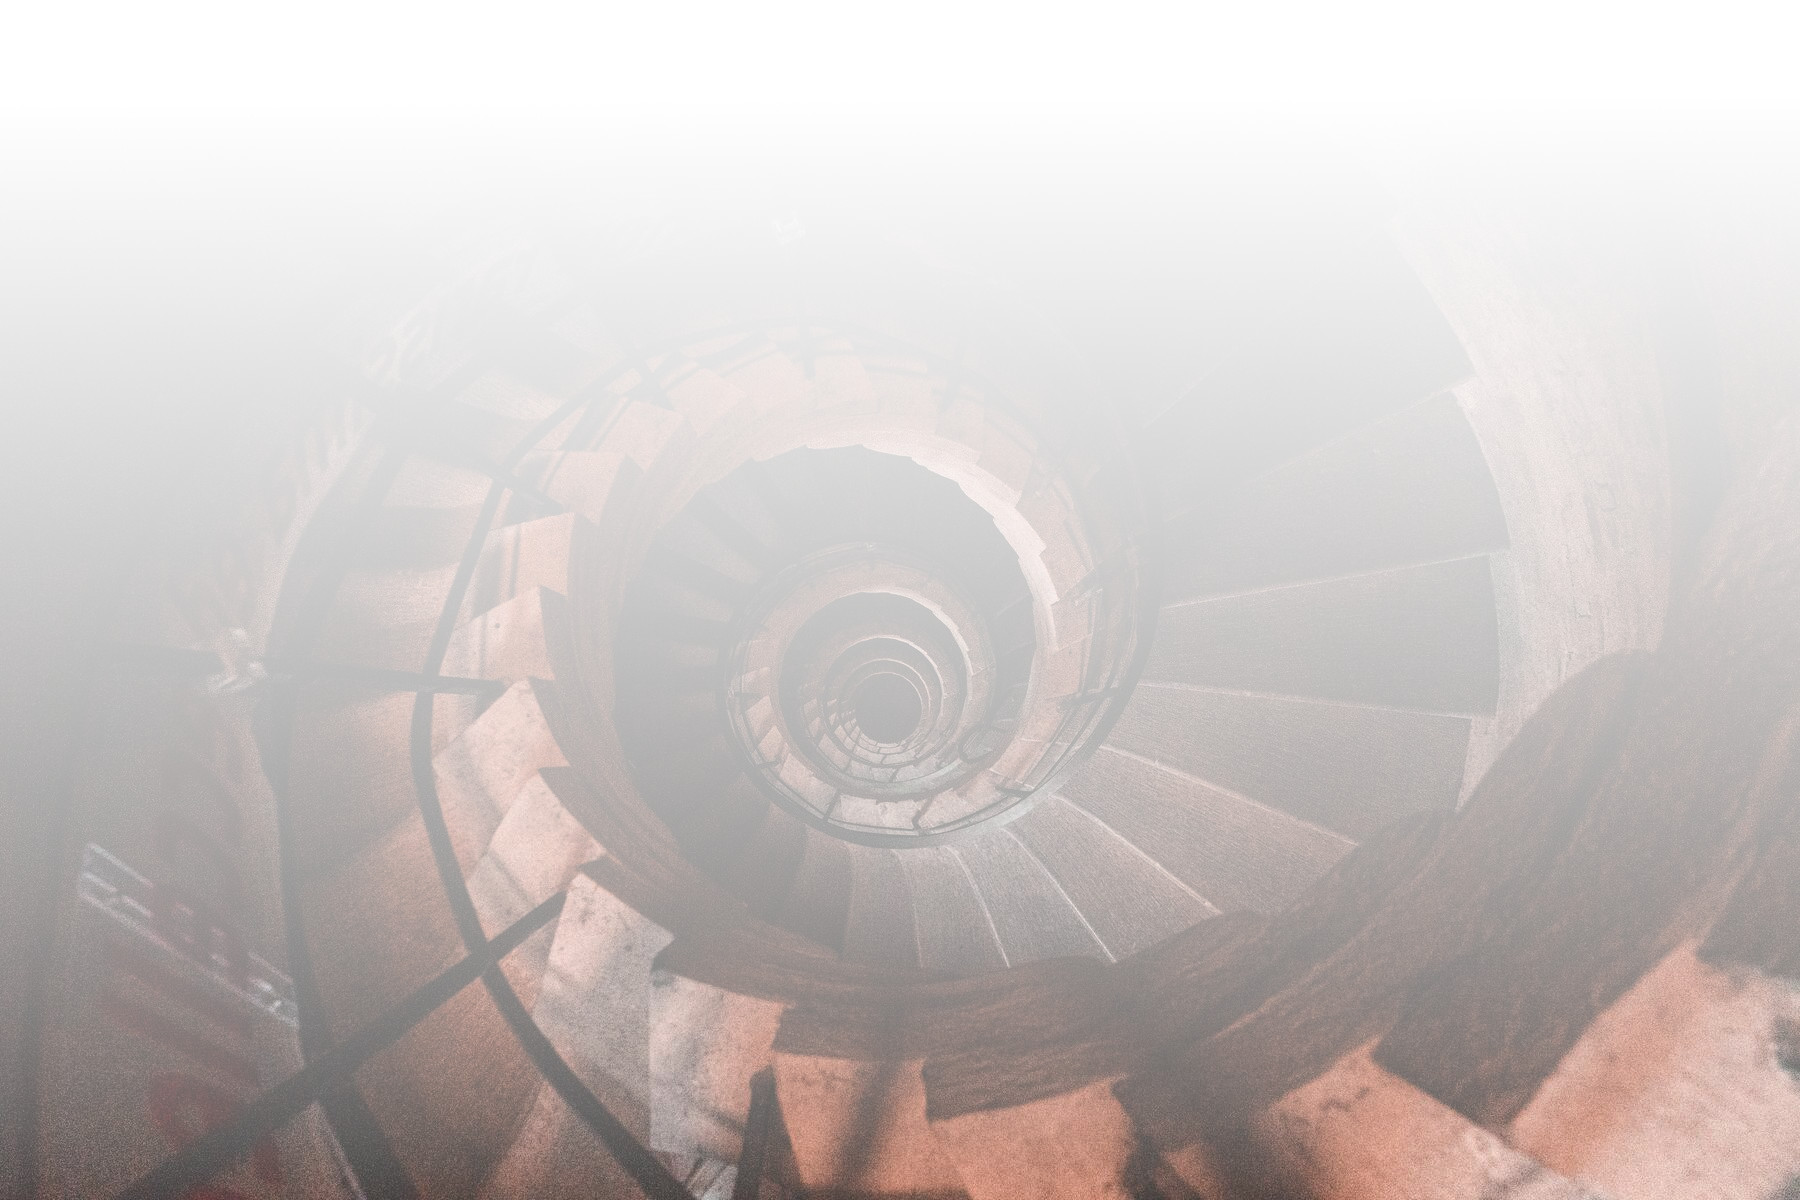
\includegraphics[width=\paperwidth]{staircase}\end{minipage}}
\begin{frame}{Transfinite methods}
  The current presentation of algebraic geometry hinges on:
  \begin{itemize}
    \item large structures: classes, large categories, universes, \ldots
    \item powersets
    \item law of excluded middle
    \item axiom of choice
  \end{itemize}
  \bigskip

  \subhead{despite:}
  \begin{enumerate}
    \item subject matter (in part) very concrete
    \item practical computer algebra systems for computations
    \item well-developed constructive algebra
  \end{enumerate}
\end{frame}}

\begin{frame}{Formalizing algebraic geometry}
  \bigskip
  \bigskip
  \bigskip
  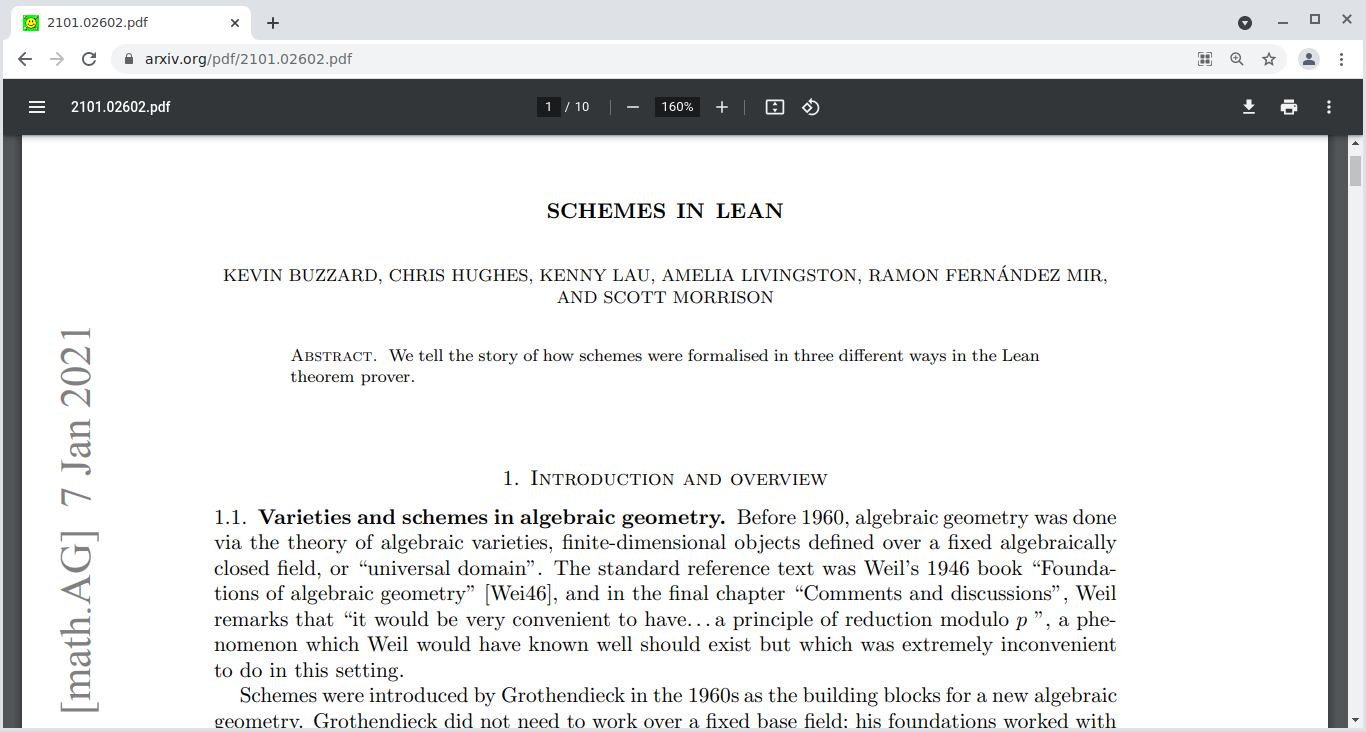
\includegraphics[width=\textwidth]{schemes-in-lean2}

  \vspace*{-17em}
  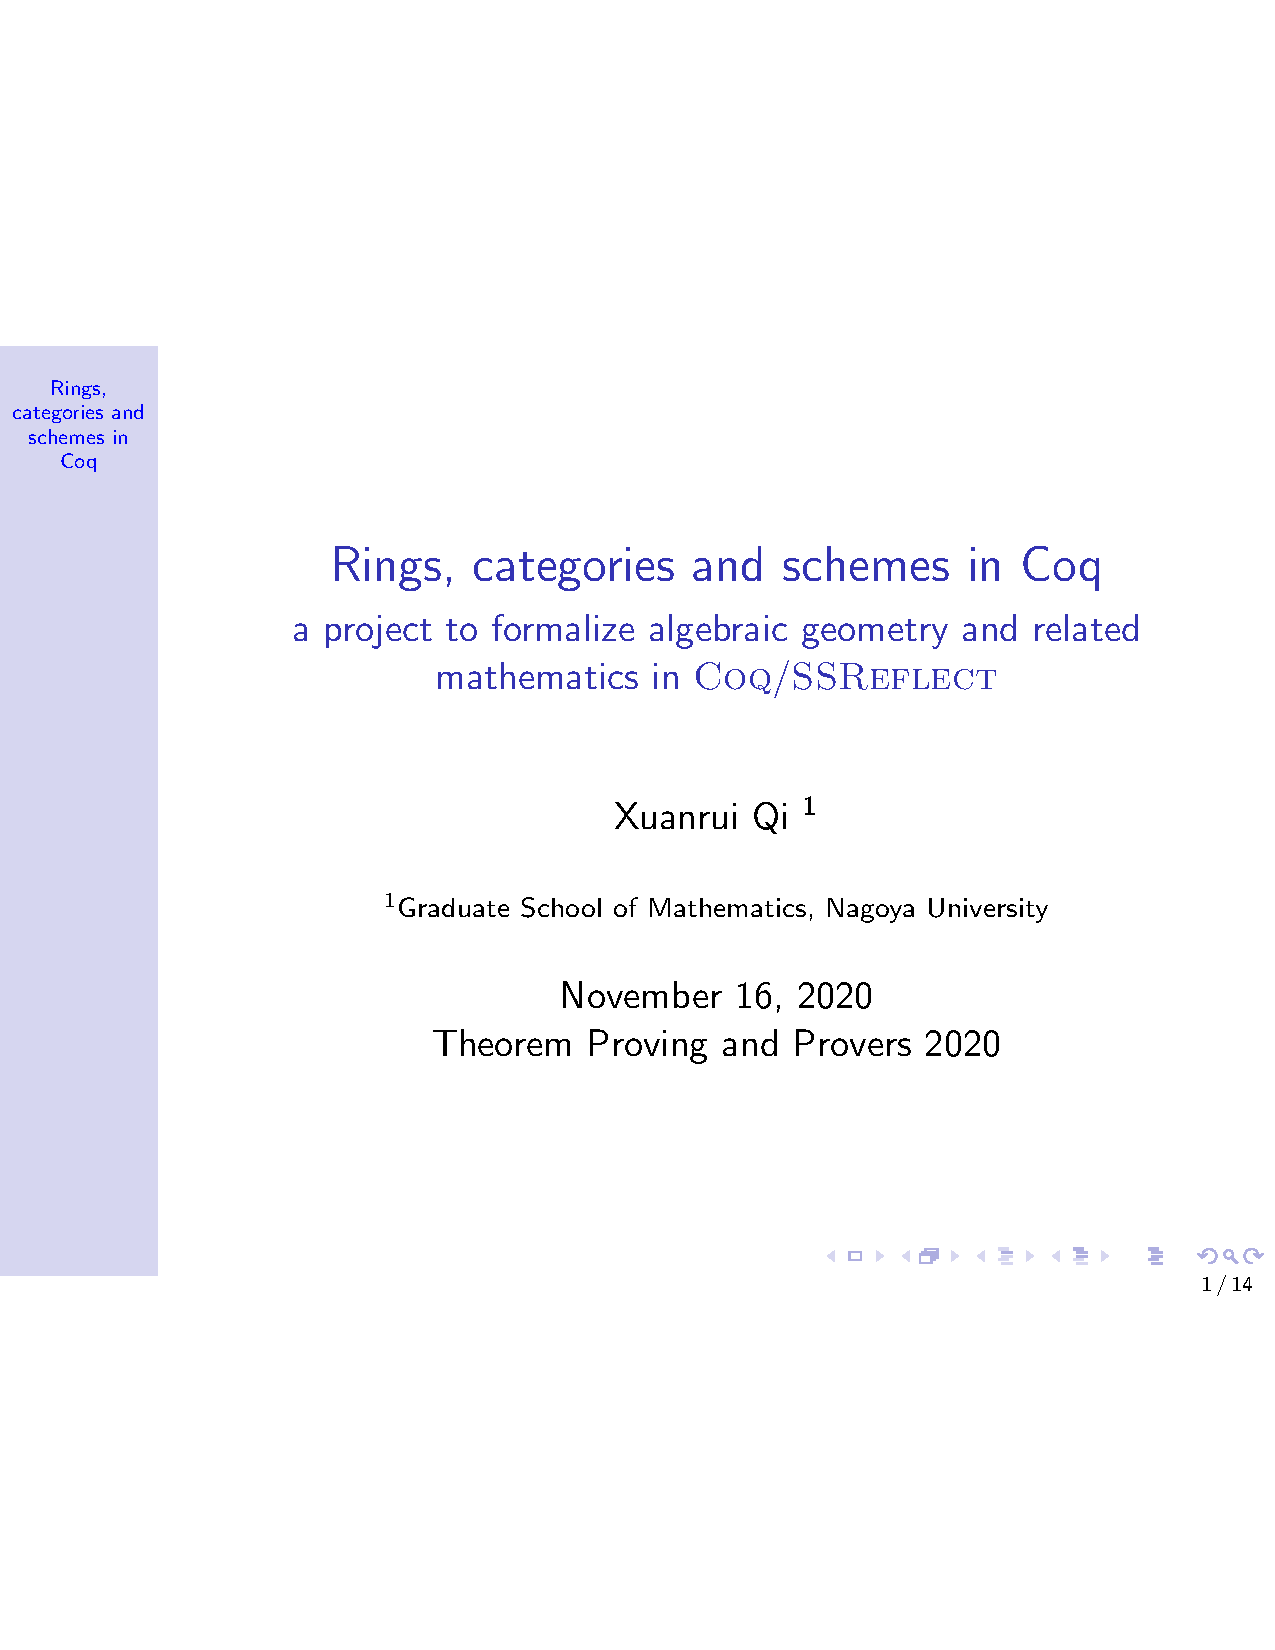
\includegraphics[frame=0.1em,bb=0 170 610 625,width=0.3\textwidth]{schemes-in-coq}\hfill
  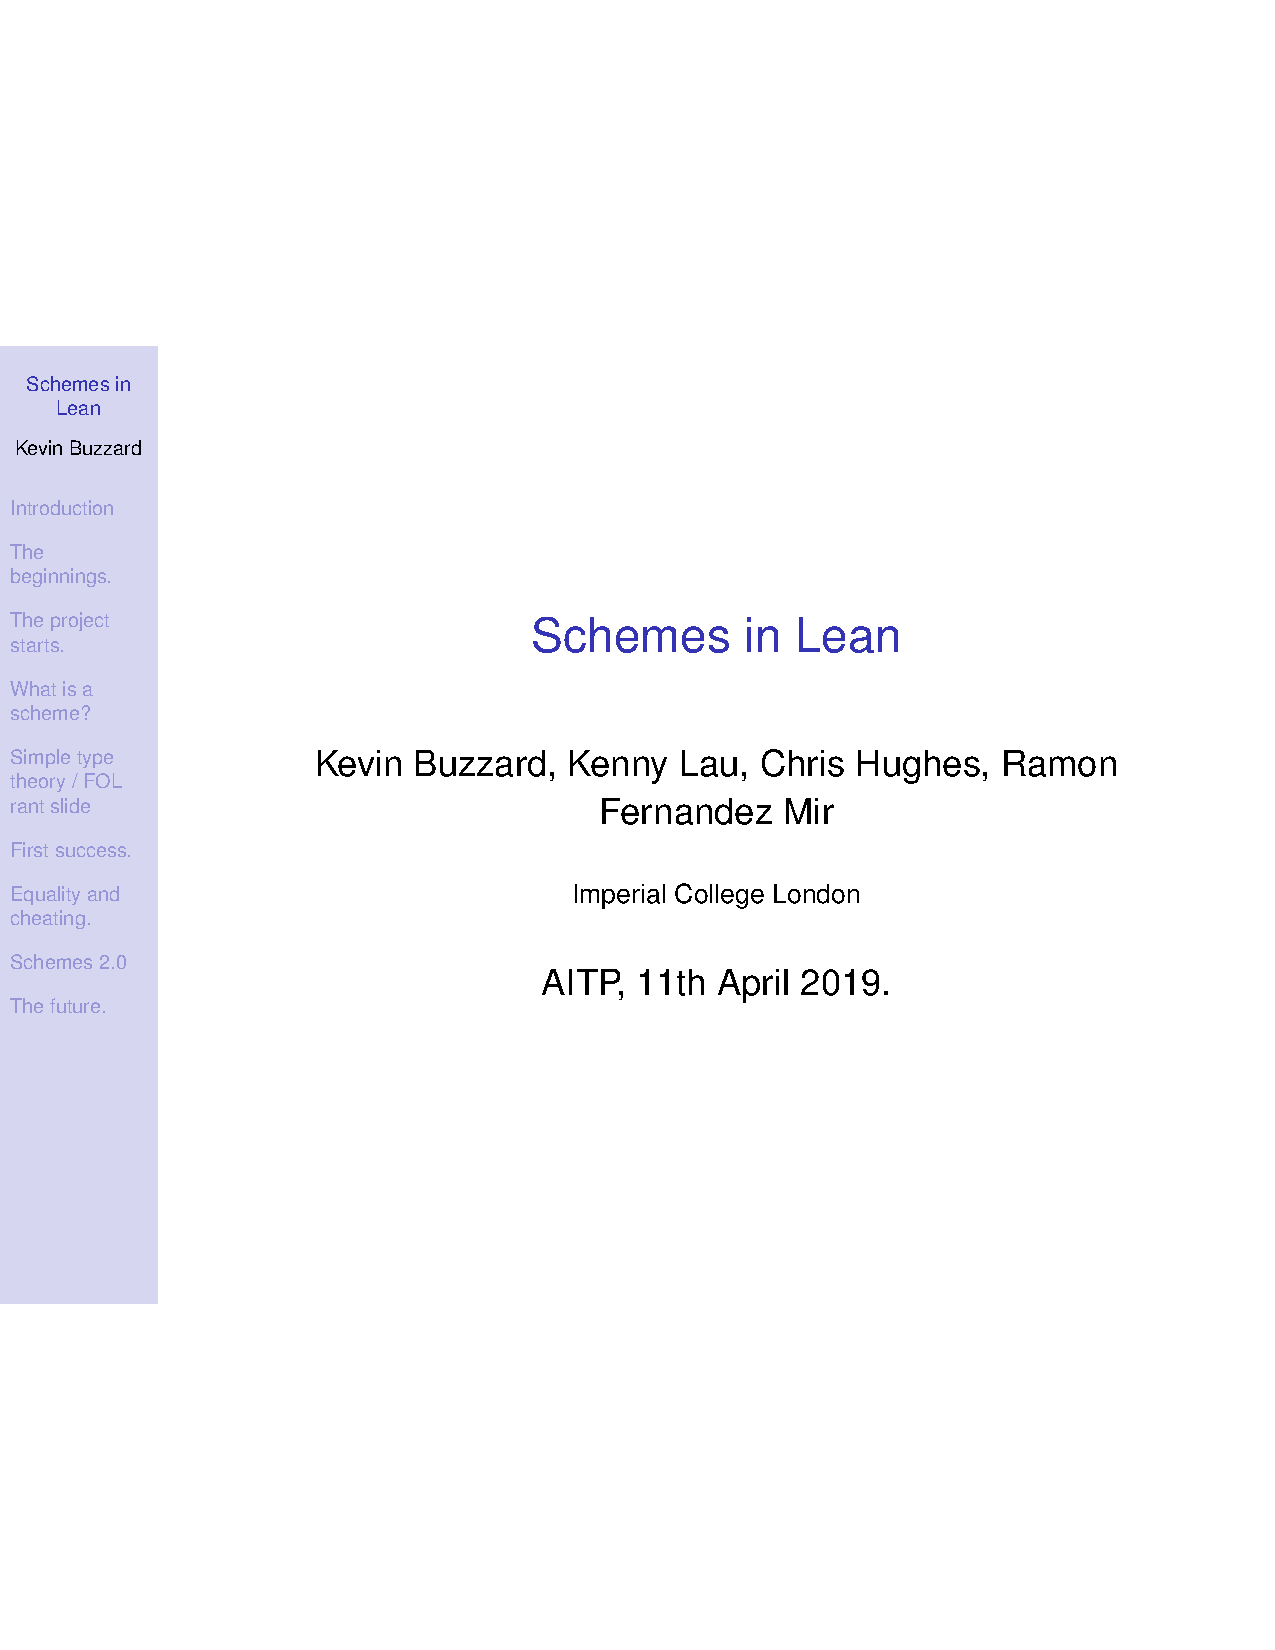
\includegraphics[frame=0.1em,bb=0 170 610 625,width=0.3\textwidth]{schemes-in-lean}
\end{frame}

\begin{frame}{A trinitarian challenge}
  \begin{center}\tiny $1^3 + \cdots + n^3 = (1 + \cdots + n)^2$\end{center}
  \vspace*{-0.6em}

  \begin{columns}
    \begin{column}{0.33\textwidth}
      \centering
      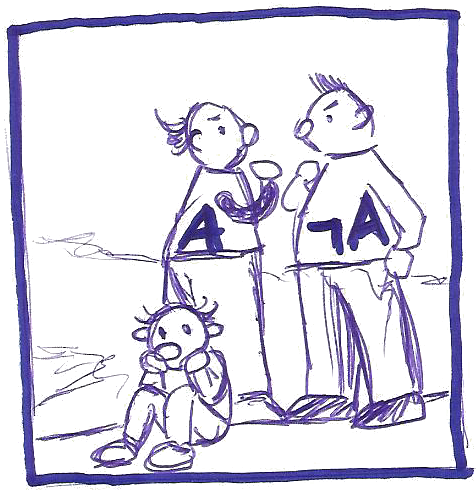
\includegraphics[height=7em]{lem}

      \hil{constructivity}
      \par
    \end{column}
    \begin{column}{0.33\textwidth}
      \centering
      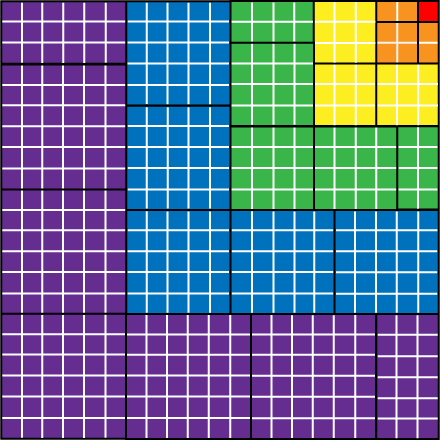
\includegraphics[height=7em]{sum-of-cubics}

      \hil{elegance}
      \par
    \end{column}

    \begin{column}{0.33\textwidth}
      \centering
      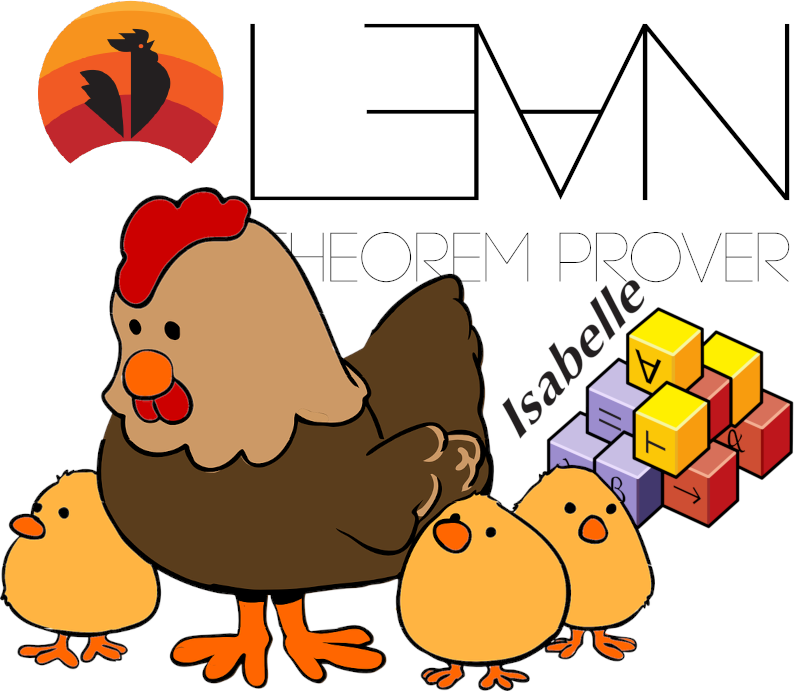
\includegraphics[height=7em]{proof-assistants}

      \par
      \hil{formalizability}
    \end{column}
  \end{columns}
  \bigskip
  \bigskip

  \subhead{Thesis}
  \centering
  Elegant mathematics lends itself to rewarding formalization.
\end{frame}

\begin{frame}{Foundational possibilities}
  \small

  \subhead{Schemes and scheme morphisms}
  \only<1-2>{
  \begin{itemize}
    \setlength\itemsep{-0.2em}
    %\item locally ringed spaces (or locales, distributive lattices, sites,
    %toposes, arithmetic universes), formal geometries
    \item locally ringed \ldots \\
    \ldots{} spaces \tabto{4cm}-- \textit{unconstructive, hard to formalize} \\
    \ldots{} locales \tabto{4cm}-- \textit{impredicative, superfluous opens} \\
    \ldots{} distributive lattices \tabto{4cm}-- \textit{need extension from basis} \\
    \ldots{} sites \tabto{4cm}-- \textit{current favorite! morphisms intricate} \\
    \ldots{} toposes \tabto{4cm}-- \textit{large structure} \\
    \ldots{} arithmetic universes \tabto{4cm}\mbox{-- \textit{a bit better;
    issue with relative spectrum}}
    \item formal geometries \tabto{4cm}-- \textit{can be regarded as sites}
    \item functor of points \tabto{4cm}-- \textit{large structure, issue with
    sizes or \\ \qquad
    with schemes not of finite presentation over the base ring}
    \item formal gluing data \tabto{4cm}-- \textit{morphisms intricate}
  \end{itemize}
  \textbf{A surprise of uncertain import:}
  \pause
  Internally to the big Zariski topos of a base scheme, the Zariski spectrum of
  a finitely presented algebra does have enough points! [Cherubini--Coquand]}
  \bigskip
  \pause

  \subhead{Zariski cohomology}
  \begin{itemize}
    \setlength\itemsep{-0.2em}
    \small
    \item Čech cohomology \tabto{4.5cm}-- \textit{ad hoc, but fine for}
    \tabto{4.5cm}\phantom{--} \textit{quasicompact separated schemes}
    \item injective resolutions \tabto{4.5cm}-- \textit{hopelessly unconstructive}
    \item flabby resolutions \tabto{4.5cm}-- \textit{probably unconstructive}
    \item pointwise Kan extensions \tabto{4.5cm}-- \textit{fine!}
  \end{itemize}
  \bigskip

  \subhead{Étale cohomology}
  \textcolor{red!90}{??}
\end{frame}

\end{document}


\section{The generic model}

\subsection{The generic ring}

\begin{frame}{The generic ring}
  \visible<2->{``}Let~$R$ be a ring.\visible<2->{''} \visible<2->{-- Which ring does this phrase refer to?}

  \vspace*{-0.6em}
  \begin{center}
    \begin{tikzpicture}[ultra thick, node distance=7mm]
      \node[rectangle, rounded corners=1pt, inner sep=5pt, draw=lime!80, fill=lime!40] (a) {$\ZZ$};
      \node[rectangle, rounded corners=1pt, draw=lime!80, fill=lime!40, right=of a] (b) {$\FF_2$};
      \node[rectangle, rounded corners=1pt, draw=lime!80, fill=lime!40, right=of b] (c) {$\QQ[X]$};
      \node[regular polygon, regular polygon sides=6, draw=orange!80, fill=orange!40, right=of c, rounded corners=1pt] (d) {$\RR$};
      \node[regular polygon, regular polygon sides=5, draw=pink!80, fill=pink!40, right=of d, rounded corners=1pt, inner sep=0cm] (e) {$\O_X$};
      \visible<3->{\node[star, rounded corners=1pt, star points=10, inner
      sep=2pt, draw=purple!80, fill=purple!30, right=of e] {$\AA$};}
    \end{tikzpicture}
  \end{center}
  \vspace*{-0.6em}

  \pause
  \pause
  \pause

  \justifying
  \textbf{Thm.} For any$^\star$ property~$P$ of rings, the following are
  equivalent: \\[0em]
  \begin{enumerate}
    \item The \hil{generic ring}~$\AA$ has property~$P$.
    \item Every$^\star$ ring has property~$P$.
    \item The ring axioms entail property~$P$.
  \end{enumerate}
  \pause

  \textbf{Example A.} For any~$x,y,z \in \AA$, $x + (y + z) = (x + y) + z$.
  \pause

  \textbf{Example B.} \only<6>{Is~$1 + 1 = 0$ in~$\AA$?}%
  \pause
  \only<7->{It is \hil{not the case} that~$1 + 1 = 0$ in~$\AA$. \only<8->{But also:}} \\
  \pause
  \phantom{\textbf{Example B.}} It is \hil{not the case} that~$1 + 1 \neq 0$ in~$\AA$.
  \pause

  \textbf{Example C (Anders Kock).} The generic ring is a \hil{field}:
  \[ \forall x \in \AA\_ \bigl((x = 0 \Rightarrow 1 = 0) \Rightarrow (\exists y
  \in \AA\_ xy = 1)\bigr). \]

  \pause
  \vspace*{-0.6em}
  \hil{Hence:} When verifying a coherent sequent for all rings, can without loss of
  generality assume the field condition.
\end{frame}

\begin{frame}{A selection of noncoherent sequents}
  The \hil{generic object}~$\MM$ validates:
  \begin{enumerate}
    \item $\forall x,y \in \MM\_ \neg\neg(x = y)$.
    \item $\forall x_1,\ldots,x_n \in \MM\_ \neg \forall y \in \MM\_
    y = x_1 \vee \cdots \vee y = x_n$.
  \end{enumerate}

  The \hil{generic ring}~$\AA$ validates:
  \begin{enumerate}
    \item $\forall x \in \AA\_ (x = 0 \Rightarrow 1 = 0) \Rightarrow (\exists y \in \AA\_ xy = 1)$.
    \item $\forall x \in \AA\_ \neg\neg(x = 0)$.
  \end{enumerate}

  The \hil{generic local ring}~$\AA'$ validates:
  \begin{enumerate}
    \item $\forall x \in \AA'\_ (x = 0 \Rightarrow 1 = 0) \Rightarrow (\exists y \in \AA'\_ xy = 1)$.
    \item $\neg \forall x \in \AA'\_ \neg\neg(x = 0)$.
    \item $\forall f \in \AA'[X]_{\text{degree} > 0}\_ \neg\neg \exists x \in \AA'\_ f(x) = 0$.
  \end{enumerate}
\end{frame}

\begin{frame}{An application in commutative algebra}
  \justifying
  Let~$A$ be a reduced ring ($x^n = 0 \Rightarrow x = 0$).
  Let~$\pp$ be the \hil{generic prime ideal$^\star$} of~$A$.
  Then~$A_\pp \defeq A[\pp^{-1}]$ validates:

  {\vspace*{-1.2em}
  \setbeamercolor{block body}{bg=red!30}
  \setbeamercolor{structure}{fg=purple}
  \begin{varblock}{\textwidth}{}
    $A_\pp$ is a \hil{field}: $\forall x \in A_\pp\_ (\neg(\exists y \in A_\pp\_
    xy = 1) \Rightarrow x = 0)$.

    $A_\pp$ has \hil{$\boldsymbol{\neg\neg}$-stable equality}:
    $\forall x,y \in A_\pp\_ \neg\neg(x = y) \Rightarrow x = y$.

    \mbox{$A_\pp$ is \hil{anonymously Noetherian}.}\\[-1.2em]
  \end{varblock}}

  This observation unlocks a short and conceptual proof of Grothen\-dieck's
  \hil{generic freeness lemma} in algebraic geometry.

  \mbox{\textbf{Thm.} (baby freeness) Let~$M$ be an~$A$-module. Then~\bignumber{1}
  implies~\bignumber{3}.}

  {\small
  \begin{tabular}{@{}lc@{\ }l@{}}
    \bignumber{1} $M$ is finitely generated &($\Longleftrightarrow$&
    $M_\pp$ is finitely generated) \\
    \bignumber{2} $M$ is locally free &($\Longleftrightarrow$&
    $M_\pp$ is free) \\
    \bignumber{3} $M$ is locally free \emph{on a dense open} &($\Longleftrightarrow$&
    $M_\pp$ is \emph{not not} free) \\
  \end{tabular}\par}

  \textbf{Proof.} Elementary linear algebra over~$A_\pp$. \qed
\end{frame}

\begin{frame}{A systematic source}
  \begin{center}
    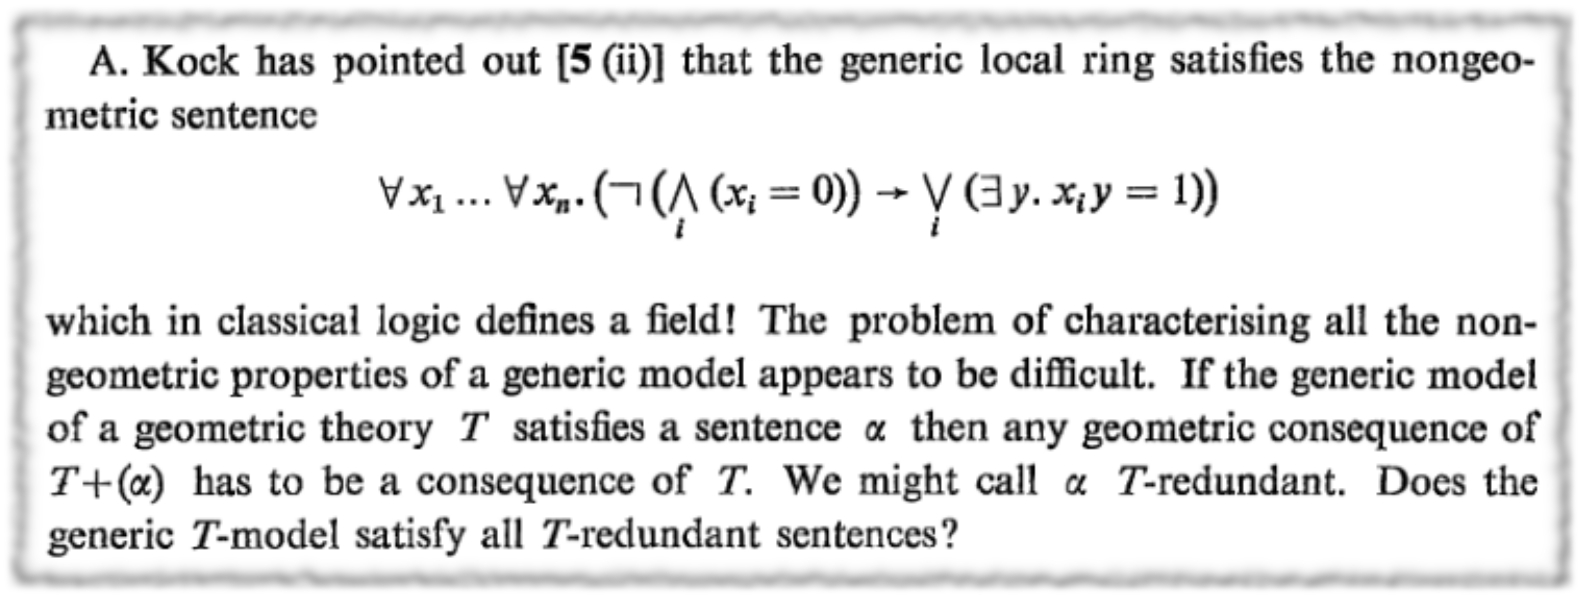
\includegraphics[width=0.8\textwidth]{wraith-some-recent-developments-in-topos-theory} \\
    \scriptsize
    Gavin Wraith. \emph{Some recent developments in topos theory.} \\ In:
    Proc.\@ of the ICM (Helsinki, 1978).
  \end{center}

  \textbf{Thm. (Nullstellensatz):} The generic~$\TT$-model~$U_T$ validates:
  For any coherent sequent~$\sigma$,
  \[
    \text{$\sigma$ holds for $U_\TT$} \quad\textcolor{purple}{\Longleftrightarrow}\quad
    \text{$\ul{\TT}/U_\TT$ proves $\sigma$.}
  \]

  \justifying
  \textbf{Thm. (universality):} The generic~$\TT$-model validates a first-order
  formula~$P$ if and only if~$P$ is intuitionistically deducible from the
  axioms of~$\TT$ and the Nullstellensatz.
\end{frame}

\begin{frame}{Arithmetic universes}
  Places where we can do mathematics (among others):
  \begin{multicols}{2}
    \begin{enumerate}
      \item $\Set$ (sets)
      \item $\Eff$ (data types) \columnbreak
      \item \mbox{$\mathrm{sSet}$ (simplicial sets)}
      \item \mbox{$\Sh(X)$ (sheaves over~$X$)}
    \end{enumerate}
  \end{multicols}
  \pause
  \vspace*{-0.6em}
  These are examples for \hil{arithmetic universes}.
  \pause

  \justifying
  \textbf{Definition.} An \emph{arithmetic universe} is a category with finite
  limits (``$\times$''), stable finite disjoint coproducts (``$\amalg$''),
  stable ef{}fective quotients (``$X/{\sim}$'') and parametrized list objects
  (``$\NN$'', ``$\mathrm{List}(X)$'').

  \textbf{Thm.} Any statement which is provable in \hil{predicative constructive
  mathematics} (no powersets, no $\varphi \vee \neg\varphi$, no
  \mbox{$\neg\neg\varphi \Rightarrow \varphi$}, no axiom of choice) is true in any
  arithmetic universe.
  \pause

  Further examples:

  \begin{enumerate}
    \addtocounter{enumi}{4}
    \item the \hil{initial} arithmetic universe
    \item the \hil{classifying} arithmetic universe for the theory of rings
  \end{enumerate}
\end{frame}

\end{document}
